\chapter{Problemfelder innerhalb des Change Managements}
\label{problemfields}

% - erster Hauptteil der Arbeit
% - Herausarbeitung von Veränderungsprozessen und Problemfelder innerhalb der DT

Nach den theoretischen Ausführungen der vorangestellten Kapiteln soll nun inhaltlich auf den ersten Hauptschwerpunkt der vorliegenden Arbeit eingeführt werden. Um in \ref{agilepractices} eine Reihe agiler Methoden hinsichtlich ihrer Anwendbarkeit in Problemfeldern der Digitalen Transformation zu evaluieren, müssen Letztere zunächst erarbeitet werden. Dafür soll ein systematisches Literaturreview (\gls{SLR}) von Studien und Fallstudien zum Thema der Digitalen Transformation in Großunternehmen vorgenommen werden. Dadurch hat dieses SLR ebenfalls den Charakter einer \textit{Metastudie}\footnote{Studie, bei der die Ergebnisse verschiedener Untersuchungen bzw. Studien zu einer bestimmten Thematik verglichen, zusammengefasst und nach bestimmten Vorgaben bewertet werden, Definition nach enzyklo.de, online: \url{http://www.enzyklo.de/Begriff/Metastudien}}. Aus dieser werden zunächst Veränderungsprozessmuster innerhalb des Transformationsprozesses  zusammengefasst.  Zusätzlich werden auf Grundlage dessen eine Reihe von problematischen Schwerpunkten erarbeitet. Nachfolgend soll zunächst das methodische Vorgehen im aktuellen Kapitel geschildert werden. Es schließt sich eine gesonderte Übersicht der erschlossenen Literatur an, auf dessen Grundlage  die Ergebnisse aufgeführt werden.  Das nachfolgende, erste Literaturreview wird im folgenden durch das Akronym \textit{SLR 1} abgekürzt.

\section{Methodisches Vorgehen}
\label{problemfields:methods}

% - genaue Darstellung über Vorgehen in der SLR + Metastudie
% - Suchmethodik, Keywords, Kriterien, Auswahlprozes ...
% - https://docs.google.com/document/d/1wzYRearLcVTlKJxPp6Mz5U860VoXzkNX7armGeCoxt4/edit

Nachfolgend soll das genaue methodische Vorgehen des ersten systematischen Literaturreviews vorgestellt werden. Vor der eigentlichen Suche nach Fallstudien bzw. relevanter Literatur zum Thema der Digitalen Transformation, wurde eine einheitliche Suchstrategie aufgestellt. Diese wird in \ref{fig:suchstrategie} dargestellt. 

\begin{figure}[H]
	\centering
	\fbox{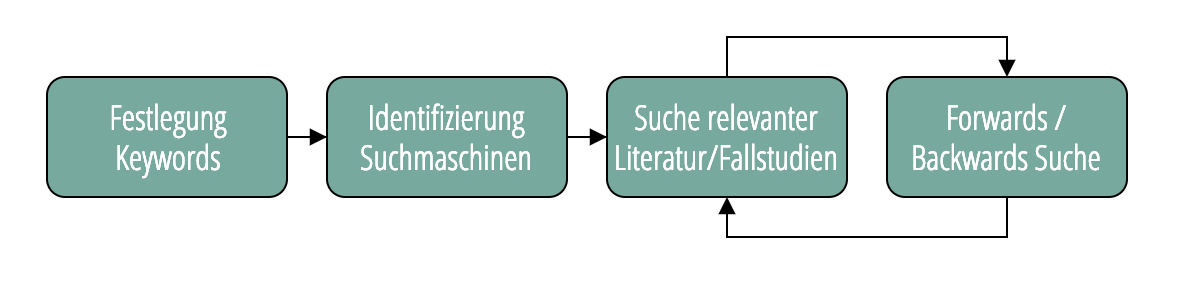
\includegraphics[width=0.8\linewidth]{pics/suchstrategie}}
	\caption[Suchstrategie des SLR]{Suchstrategie des SLR (eigene Darstellung)}
	\label{fig:suchstrategie}
\end{figure}

Wie der Abbildung zu entnehmen wurden zunächst \textit{Keywords} für die  Literatursuche festgelegt. Diese sind nach einer ersten Probesuche zunehmend angepasst worden, bis eine zufriedenstellende Eingabemaske erzielt werden konnte. Da in der Suche englische  und deutsche Literatur eingeschlossen wurde, wird im Folgenden zwischen englischen und deutschen Keywords unterschieden. In \ref{tab:keywordsslr1} werden nachfolgend die \textit{Keyword-Suchketten} aufgeführt, die in sämtlich genutzten Literatursuchmaschinen verwendet wurden. Die Syntax der Suchketten kann dabei  von Suchmaschine zu  Suchmaschine variieren, die Übersicht dient der Allgemeinheit.

\begin{table}[ht]
	\centering
	\caption{Übersicht Keyword-Suchketten SLR 1}
	\begin{tabular}{|p{7cm}|p{7cm}|}
		\hline
		\textbf{Deutsche Keywords}& \textbf{Englische Keywords} \\
		\hline
		digitale+transformation+fallstudie OR digitalisierung+fallstudie   & digital+transformation+case OR digitalization+case \\
		\hline
	\end{tabular}
	\label{tab:keywordsslr1}
\end{table}

Weiter wurden im Vorfeld relevante Literatursuchmaschinen identifiziert. Dabei wurde darauf geachtet, dass überwiegend Suchmaschinen mit Zugang zu technischer und teilweise wirtschaftlicher Relevanz gewählt wurden. Grundsätzlich sind überwiegend Datenbanken mit vorhandenem Online-Zugang genutzt worden. \ref{tab:suchmaschinenslr1} zeigt hierbei  eine Übersicht der genutzten Suchmaschinen mit Angabe der insgesamt gefundenen Literatur.

\begin{table}[ht]
	\centering
	\caption{Übersicht Literatursuchmaschinen SLR 1}
	\begin{tabular}{|p{5cm}|p{7cm}||p{3cm}|}
		\hline
		\textbf{Datenbank/Bibliothek}& \textbf{URL} &  \textbf{Treffer Keywords  (summiert)} \\
		\hline
		IEEE Xplore & \url{https://ieeexplore.ieee.org} & 770 \\
		(Online) - Bibliothek Hochschule Harz & \url{https://opac.lbs-magdeburg.gbv.de/DB=4/LNG=DU} & 6 \\
		(Online) - Bibliothek Technische Universität Berlin  & \url{https://www.ub.tu-berlin.de/literatur-suchen}& 1 \\
		Google Scholar &  \url{https://scholar.google.de}  & 26.800 \\
		Scopus & \url{https://www.scopus.com} & 4.347 \\
		ResearchGate & \url{https://www.researchgate.net} &Keine Angabe vorhanden \footnotemark \\ 
		ACM Digital Library & \url{https://dl.acm.org} & 174.857 \\
		\hline
	\end{tabular}
	\label{tab:suchmaschinenslr1}
\end{table}

\footnotetext{\textit{ResearchGate} bietet keine Funktion zur Angabe der kompletten Treffer-Zahl}

Des Weiteren beinhaltete der vorgenommene Suchprozess eine sogenannte \textit{Forwards - und Backwards-Suche}. Demzufolge wurden mithilfe der bereits gefundenen Fallstudien weitere, zitierte Studien erschlossen (Backwards). Ebenso wurden mithilfe der Suchmaschinen, insoweit die Funktion bereitgestellt wurde, Fallstudien oder Literatur gesucht, die von den gefunden Fallstudien zitiert wurden (Forwards). So konnte eine große Menge von potentiellen Fallstudien  gefunden werden.

Die Angaben zu den Literatur-Treffern in den einzelnen Suchmaschinen zeigt klar, dass eine weitere Filterung vorgenommen werden musste. Dafür wurde ein \textit{Auswahlprozess} definiert, um nur relevante Fallstudien für die folgenden Untersuchungen zu inkludieren. Dieser wird in \ref{fig:auswahlprozess} dargestellt.

\begin{figure}[H]
	\centering
	\fbox{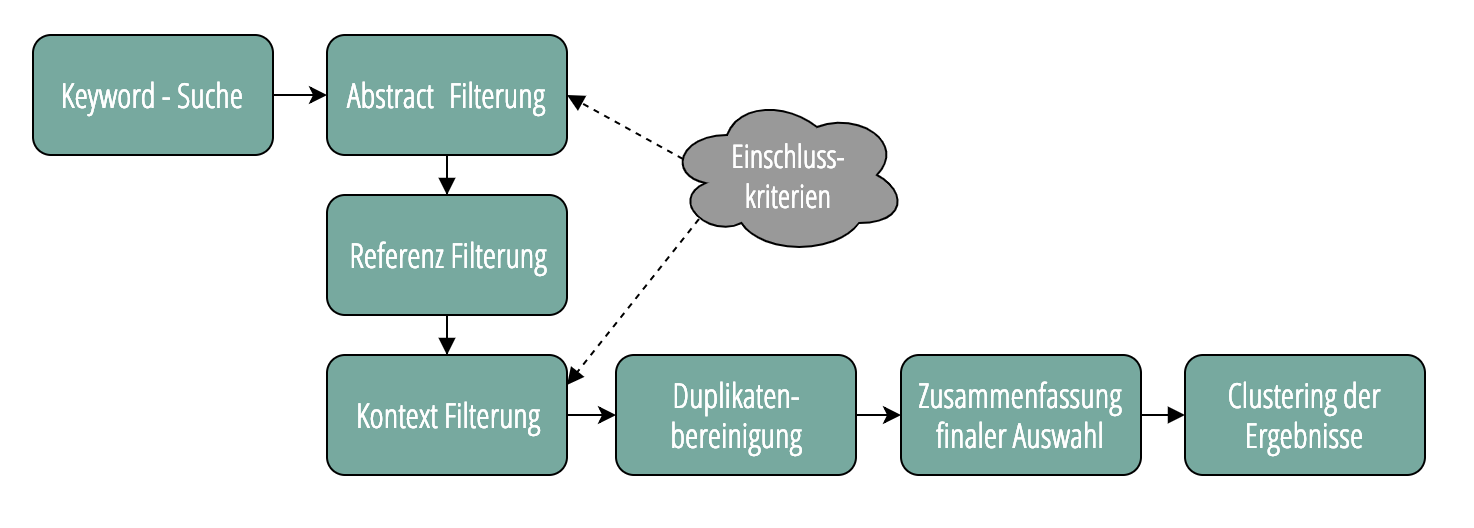
\includegraphics[width=0.8\linewidth]{pics/auswahlprozess}}
	\caption[Auswahlprozess des SLR]{Auswahlprozess des SLR (eigene Darstellung)}
	\label{fig:auswahlprozess}
\end{figure}

Um der großen Menge an Literatur zu begegnen und zu filtern, wurden eine Reihe von Schritten durchgeführt. Wie der \ref{fig:auswahlprozess} zu entnehmen, wurde für die gesamte aus der Keyword-Suche ermittelten Literatur zunächst eine Reihe von \textit{Ein - und Ausschlusskriterien} durchlaufen. Diese bezogen sich zunächst nur auf den Abstract. Sind beispielsweise wesentliche Keywords gar nicht erst vorhanden, wird die betrachtete Literatur verworfen. Weiterhin wurde überprüft, ob auf eine referenzielle Unverfälschtheit geschlossen werden kann. Dies bedeutet, dass solche Literatur nicht benutzt wird, die augenscheinlich nur eine Kopie einer bereits gefundenen ist; und zwar in dem Zusammenhang, als das sie gegenseitig im Literaturverzeichnis vorkommen. An dieser Stelle sei gesagt, dass dieser Fall sehr vermindert aufgetreten ist. 

Des Weiteren wurden die Ein - und Ausschlusskriterien auf den eigentlichen Inhalt jeder Literatur angewendet. Im Anschluss wurden eine weitere Duplikatenbereinigung durchgeführt. Als Ergebnis dieser Filterungsschritte konnte eine viel kleinere Stückzahl an Fallstudien gewonnen, diese zusammengefasst und geclustert werden.

Im Folgenden soll auf die genutzten Ein - und Ausschlusskriterien eingegangen werden. \ref{tab:criteriaslr1} zeigt eine Übersicht der genutzten Kriterien. Grundsätzlich wurde keine Einschränkung in Bezug auf die Nationalität des beschriebenen Unternehmens gemacht. Ebenso gab es keine Beschränkung auf die Branche. Im Bezug auf die \textit{Empirik} wurden nur Fallstudien oder Studien zugelassen. Ebenso mussten alle Objekte eine klare Methodik vorweisen. Demzufolge musste jeweils klar erkenntlich sein, was untersucht wurde und mit welchen wissenschaftlichen Mitteln. Inhaltlich mussten sich die (Fall-)Studien auf die  Implementation einer Digitalen Transformation in einem Großunternehmen beziehen. Studien zu KMU wurden  nur dann einbezogen, wenn ein klarer Bezug zu einem größeren Kontext gegeben war, beispielsweise durch Ausführungen für eine mögliche Skalierung der gefundenen Ergebnisse. Außerdem wurden nur solche Fallstudien inkludiert, die gesamtorganisationale Schwerpunkte setzen. Dies bedeutet, dass nicht nur auf die Implementation einzelner Technologien, wie beispielsweise \textit{Big Data} eingegangen werden sollte. Ein Bezug auf  das gesamte Unternehmen muss klar erkenntlich sein. Hinsichtlich der gewählten Sprache musste die Literatur auf deutsch oder englisch sein. Das Veröffentlichungsdatum durfte nicht vor dem Jahr 2014 liegen, um eine gewisse Aktualität zu gewährleisten.

\begin{table}[ht]
	\centering
	\caption{Ein - und Ausschlusskriterien SLR 1}
	\begin{tabular}{|p{4cm}|p{8cm}|}
		\hline
		\textbf{Kriterium}& \textbf{Erklärung}  \\
		\hline
		Empirik & Literatur muss eine Fallstudie oder Studie sein \\
		Wissenschaftlichkeit & Methodik der  Fallstudie oder Studie muss klar erkennbar sein \\
		Kontext & inhaltlich Digitale Transformation in Großunternehmen; Mittelständische nur dann, wenn relevant für größeren Kontext \\
		Allgemeinheit & keine Spezifität von einzelnen technischen Implementationen, Gesamtorganisationaler Kontext muss vorhanden sein \\
		Sprache & deutsch oder englisch \\
		Aktualität & ab 2014 - heute  \\
		\hline
	\end{tabular}
	\label{tab:criteriaslr1}
\end{table}

Durch die genutzten Ein - und Ausschlusskriterien konnte die große Menge an Literatur auf eine kleine Gruppe relevanter Fallstudien und Studien im Themenfeld der Digitalen Transformation von Großunternehmen heruntergebrochen werden. Insgesamt konnten \textit{23} Literaturobjekte gefunden werden. Diese beinhalten zusammen rund \textit{200} Fallstudien zu Großunternehmen in verschiedenen Bereichen.

\section{Literaturübersicht}

% - Fallstudien
% - tabellarische Darstellung (https://docs.google.com/document/d/1caHZ-pLGa\_L-TfO4nOh2zZLdAa5nazKaoUZDeDmN90M/edit)
% - Inhaltsangabe jeder Arbeit (Zusammenfassung)

Nachfolgend soll eine kleine Übersicht der gefundenen und gefilterten Literatur gegeben werden, die für die weiteren Untersuchungen verwendet wurden. Eine große Übersicht der  Bücher, wissenschaftlichen Artikeln u. a. findet sich in \ref{tab:overviewliterature1} und \ref{tab:overviewliterature1-2} im Anhang. Diese beinhaltet neben Autor und Titel jeder Publikation eine kurze Übersicht zum Untersuchungsgegenstand.

Wie im vorangestellten Abschnitt bereits aufgeführt, wurden insgesamt 23 (Fall-) Studien ausgewertet. Jede eingeschlossene Publikation muss zumindest in ausgewählten Abschnitten Fallstudien zum dargestellten Thema beinhalten. Nachfolgend soll für jede eine kurze inhaltliche Beschreibung gegeben werden.

\citeA{muchna_aspekte_2018} thematisieren in ihrer Arbeit grundsätzliche Aspekte des Zusammenwirkens von Innovations- und Change Management. Gesondert im 7. Kapitel wird eine Fallstudie der Digitalen Transformation des Deutschen Banksektors  beschrieben. Es wird auf aktuelle Herausforderungen, Chancen und Best Practices im Bezug auf die Digitalisierung für diese Branche eingegangen.

Ein sehr übersichtlichen Beitrag zu Fallstudien innerhalb der Digitalen Transformation von Großunternehmen stellen \citeA{gassmann_digitale_2016} in ihrem Buch bereit. Besonders im zweiten Teil werden gleich 11  Fallstudien zu dieser Thematik dargestellt. Es wird systematisch auf Erfolgsfaktoren und Handlungsanweisungen für  eine erfolgreiche Digitale Transformation hingewiesen, jedoch auch auf Hürden und Probleme eingegangen.

Einen weiteren Fall beschreiben \shortciteA{chanias_digital_2018} in ihrer Arbeit. Es geht zwar hierbei um die Digitale Transformation eines mittelständischen, europäischen Anbieter im Finanzwesen, jedoch werden die Ergebnisse weiterführend in Form von allgemeinen Problematiken und Handlungsempfehlungen auf einen großen Kontext geschlossen. Damit gelten die Ein - und Ausschlusskriterien (vgl. \ref{problemfields:methods}, ab S. \pageref{problemfields:methods}) als erfüllt.

Eine ganze Reihe von Fallstudien präsentieren \citeA{urbach_digitalization_2018} in ihrer Publikation. Es werden gleich 21 Fälle der Digitalen Transformation von Großunternehmen präsentiert. Hierbei wurde sehr systematisch vorgegangen und  wiederkehrend auf Probleme, Lessons Learned und Best Practices eingegangen.

Insgesamt neun internationale Fälle bietet das Werk von \citeA{gartner_fallstudien_2018}. Interessant ist hier, dass in allen Fällen direkt auf den Einfluss des Mitarbeiters als Menschen eingegangen wurde.

\citeA{oswald_digitale_2018} beschreiben im vierten Teil ihres Buches vier Fallstudien aus dem deutschsprachigen Raum. Es wird außerdem angegeben, dass Erfahrungen aus 59 Unternehmen und die Erhebung einer Studie von 650 Organisationen in der Automobilbranche für die Erstellung der Fallstudien eingeflossen sind.

Eine große Studie führten außerdem \shortciteA{hoberg_skills_2017} durch und veröffentlichen die Ergebnisse in ihrer Arbeit. Insgesamt wurden 116 Vertreter von Unternehmen aus 18 Ländern befragt. Die Ergebnisse zeigen klare  Trends in der Implementation der Digitalen Transformation und weisen auch vermehrt auf Probleme hin.

Eine weitere Studie führten \citeA{solis_2017_2017} durch. Insgesamt wurden 528 Offizielle von Unternehmen aus fünf großen Industriestaaten befragt. Die Ergebnisse zeigen gegenwärtige Entwicklungen innerhalb der Digitalen Transformation der befragten Unternehmen.

\citeA{kremins_2018_2018} führte eine Studie innerhalb der internationalen Reisebranche durch. Insgesamt wurden rund 200 Unternehmen befragt. Als Ergebnisse werden Probleme und Handlungsempfehlungen dargestellt.

Im Bezug auf die Handelsbranche stellten \shortciteA{heinemann_digitale_2016} insgesamt 15 Fallstudien von internationalen Großunternehmen in dieser Branche zusammen. Es wird systematisch auf Probleme und Handlungsempfehlungen eingegangen.

\citeA{nowik_promoting_2018} fasst in seiner Arbeit die Ergebnisse einer Studie mit acht schwedischen Großunternehmen aus der Finanzbranche zusammen. Es wird schwerpunktmäßig auf Probleme und Gründe eingegangen, warum bestimmte Firmen im Transformationprozess zunehmend hinter ihrer Konkurrenz liegen.

Im Transformationswerk des Jahres 2016 stellen \citeA{buhse_transformationswerk_2016} eine Studie mit 1060 Vertretern von deutschen Groß - und mittelständischen Unternehmen vor. Es wird  verstärkt auf Problematiken im Transformationsprozess, aber auch auf Treiber und Handlungsweisungen eingegangen.

Eine große Fallstudie präsentiert \citeA{wautelet_impact_2017} in seiner Arbeit. Es wird zunächst auf die Notwendigkeit der Digitalen Transformation des dargestellten Unternehmens, dann auch auf Probleme und Lessons Learned eingegangen.

Die Ergebnisse von insgesamt 82 Fallstudien fasst die Arbeit von \citeA{weber_digital_2015} zusammen. Alle betrachteten Unternehmen kommen aus dem Fertigungs-,  Dienstleistungs-,  sowie dem Informations - und Kommunikationstechnologie-Sektor (IKT). Es werden wichtige Handlungsfelder und Grundlagen für den Erfolg der Digitalen Transformation dargestellt.

Insgesamt drei Medienkonzerne aus dem deutschsprachigen Raum stellt \shortciteA{hess_options_2016} in seiner Publikation dar. Es wird auf Probleme  und wichtige Treiber der Transformation in diesen Unternehmen eingegangen.

Eine weitere Studie zum Status der Digitalen Transformation in Deutschland stellt \citeA{depiereux_studie_2018} vor. Insgesamt wurden 2000 Unternehmen befragt. Es wird auf wichtige gegenwärtige Probleme eingegangen.

\citeA{buxmann_digitalisieren_2016} beschreiben in ihrer Arbeit die Ergebnisse einer Studie mit 103 Großunternehmen aus der deutschen Maschinen- und Anlagenbau-, Automotive- sowie Logistik/Transport-Branche. Es wird darauf hingewiesen woran es zunehmend im Transformationsprozess mangelt und an welchen Punkten für einen erfolgreichen Wandel gearbeitet werden muss.

Insgesamt fünf Fallstudien aus dem deutschsprachigen Raum zeigen \citeA{berghaus_2016} in ihrer Veröffentlichung. Es werden systematisch Erfahrungsberichte aufgezeigt. Interessant ist hier die Erkenntnis, dass oftmals ein klares  Ziel beim Transformationsprozess fehlt.

Eine Übersicht im Bezug zur Digitalen Transformation aller 30 DAX-Unternehmen stellen \citeA{kawohl_digitale_2016} vor. Es wird auf den aktuellen Status der Unternehmen im Transformationsprozess eingegangen, sowie  auf  Probleme und Handlungsweisungen.

\shortciteA{beule_digital_2019} thematisieren in ihrer  Arbeit die Erkenntnisse von sechs Fallstudien von internationalen Unternehmen in der Radiobranche. Das Ziel war hierbei, Problemfelder zu identifizieren und Lösungsvorschläge zu präsentieren.

Im dritten Teil ihrer Arbeit stellen \citeA{oswald_shaping_2017} insgesamt drei  Fallstudien zu Großunternehmen vor. Es wird  auf die Bedeutung der Transformation, sowie im einzelnen auf Probleme und Handlungsempfehlungen eingegangen.

Eine weitere Fallstudie präsentieren \shortciteA{savastano_how_2018} in ihrer Arbeit. Das beschriebene Unternehmen befindet sich in der Ernährungsbranche. Es wird verstärkt auf Probleme und wichtige Lessons Learned eingegangen.

Als letzte Publikation wurde die Arbeit von \citeA{macgillavry_digital_2014} eingeschlossen. Sie beschreiben eine Fallstudie eines großen, internationalen Unternehmens aus der Logistikbranche. Es werden Herausforderungen, aber auch wichtige Handlungsempfehlungen gegeben.

Insgesamt bieten alle gefundenen und eingeschlossenen Publikationen eine sehr große Vielfalt an Erkenntnissen, die im Folgenden in zwei Schritten zusammengefasst und geclustert werden sollen.

\section{Veränderungsprozessmuster innerhalb der Digitalen Transformation}
\label{problemfields:changepatterns}

Nachdem im vorangestellten Abschnitt die  gewählte Literatur inhaltlich kurz  beschrieben wurde, sollen die Ergebnisse aller (Fall-) Studien nun zusammengefasst werden. Zunächst sollen sogenannte \textit{Veränderungsprozessmuster} erschlossen werden. Wie in \ref{introduction} bereits angeklungen, beziehen sich solche Muster auf wiederkehrende Bereiche, die innerhalb der Digitalen Transformation verändert bzw. digitalisiert werden. Alle 23 Publikationen wurden genau studiert  und die genannten Felder der Veränderung extrahiert.

Eine vollständige Auswertung darüber, welche Veränderungsprozessmuster in welcher Literatur genannt wurden, findet sich in \ref{tab:clusteringchangeprocess} im Anhang anhand einer Kreuzmatrix. Eine vereinfachte Übersicht findet sich nachfolgend in \ref{tab:clusteringvpshort}. Die Übersicht zeigt den Versuch eines Clusterings, d. h. einer Zusammenfassung der Nennungen gleichartiger  Veränderungsprozessmuster. 

\begin{table}[ht]
	\centering
	\caption{Auswertung Clustering Veränderungsprozessmuster (kurz)}
	\begin{tabular}{|c|c|}
		\hline
		\textbf{Veränderungsprozessmuster}& \textbf{Anzahl Nennungen} \\
		\hline
		Einführung einer Multi-Kanal-Strategie   & 6  \\
		Wechsel vom Offline- zum Online-Vertrieb & 5  \\
		Erschaffung neuer digitaler Produkte     & 12 \\
		Tendenz zur Kundenorientierung           & 16 \\
		Digitalisierung des Geschäftsmodells     & 11 \\
		Digitaler Wissensaufbau im Unternehmen   & 12 \\
		Datengestützte Verbesserungsprozesse     & 5  \\
		Erzeugung eines digitalen Ökosystems     & 7  \\
		Digitalisierung von internen Prozessen   & 7  \\
		Einbindung innovativer Technologien      & 6  \\
		Aufbau technisches Sicherheitskonzept    & 4  \\
		Digitale Neuausrichtung der Organisation & 13 \\
		Innovationsförderung                     & 7  \\
		Kooperation mit externen Treibern        & 5 \\
		\hline
	\end{tabular}
	\label{tab:clusteringvpshort}
\end{table}

Insgesamt konnten \textit{14} verschiedene Felder der Veränderung durch die Digitale Transformation anhand des SLR bestimmt werden. Diese Gruppe bildet eine Auswahl von oft genannten Varianten. Mehrere, nur einmalig genannte  Veränderungen, wurden in der Auswertung vernachlässigt.

Jede Einzelne beschreibt eine Maßnahme bzw. eine Facette des vom Transformationsprozess beeinflussten Unternehmens.  Ebenfalls zeigt die \ref{tab:clusteringvpshort} die Anzahl, in wie vielen Literaturquellen das jeweilige Muster direkt genannt wurde. Oft ergaben sich diese aus den Beschreibungen über die genauen Vorhaben der Transformation. 
In vielen Fällen lässt sich der Begriff der \textit{Digitalisierung} erkennen. Dies ist durchaus nachvollziehbar, da dieser Schwerpunkt stark mit der Digitalen Transformation einhergeht (vgl. \ref{background:dt}, ab S. \pageref{background:dt}). Nachfolgend soll auf jedes Muster kurz eingegangen werden, um ein besseres Verständnis zu schaffen.

Als Erstes kann die \textit{Einführung einer Multi-Kanal-Strategie} als eine Aktion der Digitalen Transformation genannt werden. Hierbei geht es grundlegend darum, neue  Wege des Vertriebs der eigenen Produkte zu erschließen \cite[S. 242]{muchna_aspekte_2018}. Darüber erhoffe man sich, neue Schnittstellen zum Kunden zu gewinnen; gerade durch das Aufkommen des Online-Vertriebs und Sozialen Medien \cite[S. 21]{solis_2017_2017}.

Eng damit verbunden erscheint das Muster des \textit{Wechsels vom Offline- zum Online-Vertrieb}. Nicht nur, dass Unternehmen dazu neigen, neue Online - Angebote zu bieten, alte Vertriebskanäle werden teilweise komplett aufgelöst. \citeA{oswald_digitale_2018} führen in ihrer Fallstudie zur deutschen Finanzbranche beispielsweise auf, dass klassische Bankprodukte vermehrt  mit digitalen Varianten ersetzt werden (S. 146).

Dazu gehört selbstverständlich auch die \textit{Erschaffung neuer digitaler Produkte}. Kunden sind es mit dem Aufkommen neuer technischer Möglichkeiten gewohnt, digitale Produkte zu nutzen. Demnach ist ein Umdenken in diese Art der Produktentwicklung unumgänglich, beispielsweise durch das Angebot digitaler Medien \cite[S. 303]{heinemann_digitale_2016}. 

Im Bezug auf das Angebot von digitalen Produkten geht auch die steigende \textit{Tendenz zur Kundenorientierung} einher. Es wird zunehmend wichtiger, den Kunden aktiv in die Produktentwicklung zu integrieren \cite[S. 17]{depiereux_studie_2018}. Nur so erziele man ein wirkliches Kundenerlebnis und neue Anreize, Produkte verkaufen zu können, wovon betriebswirtschaftlich letztendlich der Unternehmenserfolg abhängt.

Eine andere Variante von digitalen Produkten kann auch die allgemeine \textit{Digitalisierung des aktuellen Geschäftsmodells} sein. Bietet das Unternehmen beispielsweise Dienstleistungen an, wird es zunehmend zum Trend, diese auch über eine digitale Form anzubieten. Zum Beispiel beschreiben \citeA{oswald_digitale_2018} in einer ihrer Fallstudien, wie ein Unternehmen den Verkauf von Druckluft umgestellt hat (S. 100). Nach dem Prinzip von \textit{Druckluft as a Service} wird dieser nicht mehr zu einem Festpreis verkauft, sondern der Preis kann durch neuartige Auswertungsmethoden dynamisch angepasst werden.

Zu jedem Veränderungsprozess gehört das nötige  Know-How. Demzufolge erscheint es nicht ungewöhnlich, dass der \textit{Digitale Wissensaufbau im Unternehmen} ebenfalls als oft genanntes Muster auftaucht. Die Maßnahmen in diesen Bereich fielen sehr unterschiedlich aus. Beispielsweise wurden Workshops zur Schulung neuer digitaler Fähigkeiten für alle oder einen Teil der Mitarbeiter durchgeführt \cite[S. 177]{gassmann_digitale_2016}. Teilweise wurden sogar komplett neue Teams zusammengestellt, um die Digitale Transformation gezielt zu steuern \cite[S. 139]{urbach_digitalization_2018}. Es geht grundsätzlich darum, dem Unternehmen das nötige Rüstzeug für die Transformation zu geben, sei es durch den Einkauf von Know-How oder durch interne Schulungen.

Oft genannt wurde auch die Maßnahme der kontinuierlichen \textit{Verbesserungsprozesse} (KVP). Diese sind durchaus keine neue Erfindung, im Bezug auf die geschilderten Transformationsprozesse kristallisiert sich  aber die  Besonderheit heraus, dass diese zunehmend \textit{datengestützt} ist. Durch neue technologische Möglichkeiten, wie beispielsweise \textit{Big Data}, hat man somit die Möglichkeit, Daten und Metriken zum Veränderungsprozess oder allgemein zum Unternehmen zu erheben und regelmäßige Feedback-Schleifen zu erstellen \cite[S. 8]{beule_digital_2019}.

Interne Veränderungen wurden ebenfalls mehrfach genannt. Dabei fiel oft die Begrifflichkeit der \textit{Erzeugung eines digitalen Ökosystems}. Dies bedeutet im Wesentlichen, dass interne Prozesse mit dem eigenen Leistungsangebot an Produkten stark verdrahtet werden \cite[S. 127]{heinemann_digitale_2016}. Dieses Modell kommt somit einer großangelegten Digitalen Transformation am nächsten, indem digitale Produkte geschaffen, Netzwerke gebildet und Verbindungen zwischen internem und externem Schaffen erzeugt werden. Man kann das digitale Ökosystem somit als eine Art Verknüpfung aller in diesem Abschnitt genannten Muster verstehen.

Neben der Digitalisierung  von Dienstleistungen, Produkten und generell das eigene Geschäftsmodell, gehört auch die \textit{Digitalisierung von internen Prozesses} zum Rahmen der Digitalen Transformation. Beispielsweise durch das Aufkommen von \textit{Robotic Process Automation} (RPA) oder \textit{Predictive Maintenance} erhält man komplett neue Möglichkeiten, die eigene Wertschöpfungskette, aber auch generelle unternehmensweite Geschäftsprozesse  stetig zu optimieren \cite[S. 16f.]{urbach_digitalization_2018}.

Zur generellen Definition der Digitalen Transformation gehört natürlich auch die \textit{Einbindung innovativer Technologien}. Beispielsweise wird \textit{Big Data} genutzt, um in verschiedensten Abteilungen neue Kenntnisse zu gewinnen und Innovationen voranzutreiben \cite[S. 22]{gartner_fallstudien_2018}. Oft werden diese aber auch genutzt, um die eigene IT-Infrastruktur auszubauen \cite[S. 8]{chanias_digital_2018}. Unternehmen sollen demnach stetig versuchen, gegenwärtige Trends aufzunehmen und in ihr Geschäftsmodell zu integrieren \cite[S. S. 89]{gartner_fallstudien_2018}.

Das Thema Sicherheit hat im Bereich der Digitalisierung ebenfalls eine hohe Wichtigkeit. Deswegen erscheint es nicht überraschend, dass der \textit{Aufbau eines technischen Sicherheitskonzepts} ebenfalls als ein Veränderungspunkt mehrfach genannt wurde. Wichtig erscheint vielen Unternehmen, Informationen sicher und vertrauenswürdig zu behandeln \cite[S. 8]{weber_digital_2015}. Der Bereich des Datenschutzes von Kunden-, aber auch von Mitarbeiterdaten ist ein zunehmend wichtiges Thema.

Folgender Punkt ist bereits durch die Schaffung eines digitalen Ökosystems angeklungen. Trotzdem ist eine \textit{digitale Neuausrichtung der Organisation} weiterhin erwähnenswert. In einer Reihe von Fallstudien wurden gesonderte Umstrukturierungen der IT-Abteilung genannt \cite[S. 393]{urbach_digitalization_2018}.  Teilweise wurden auch eigene Divisionen für den Transformationsprozess geschaffen \cite[S. 8]{beule_digital_2019}, aber auch komplette Organisationen umgestellt \cite[S. 4]{kawohl_digitale_2016}. Letzteres steht auch im Zusammenhang mit denen im \ref{background:agileorganisation} geschilderten Beispielen. Es ginge grundsätzlich darum, die Organisation bereit für anstehende Veränderungen zu machen \cite[S. 31]{berghaus_2016}

Um wettbewerbsfähig zu bleiben, setzen immer mehr Unternehmen auf eine stetige \textit{Innovationsförderung}. Durch Kooperationen, gezieltes Management oder die Einrichtung von Innovationszentren soll das Schaffen neuer Ideen zunehmend gefördert werden \cite[S. 33]{buxmann_digitalisieren_2016}. Man erhoffe sich so eine Entstehung einer Innovationskultur im Unternehmen.

Als letzter, mehrfach genannter Veränderungspunkt soll die \textit{Kooperation mit externen Treibern} genannt werden. Hierbei geht  es nicht nur um die Bestellung von externen Beratern beim Veränderungsprozess, sondern auch um die direkte Kooperation mit \textit{Start-Ups} oder einer eigenen \textit{Open Source Community} \cite[S. 139]{urbach_digitalization_2018}. Man erhoffe sich hierdurch stärkende Einflüsse von außen, ohne große Anstrengungen ins eigene Wissensmanagement stecken zu müssen. Dieses Muster kann teilweise als Gegenentwurf zum digitalen Wissensaufbau gesehen werden, wobei Symbiosen auch denkbar sind \cite[S. 154]{urbach_digitalization_2018}.

Die dargestellten Veränderungsmuster lassen erahnen, dass es eine Vielzahl von Veränderungen innerhalb des Transformationsprozesses geben kann. Interessant ist hierbei, dass die \textit{Tendenz zur Kundenorientierung} am meisten genannt wurde. Dies lässt erahnen, dass viele Unternehmen in diesem Thema das größte Potenzial sehen, um neue Geschäftsbereiche und Produktangebote zu erschließen.

Die erarbeiten Muster der Veränderung werden in der Erstellung von Best Practices (vgl. \ref{agilepractices}, ab S. \pageref{agilepractices}) teilweise nochmal aufgegriffen. Nachfolgend sollen nun bestimmte Problemfelder in den getroffenen  Veränderungen erarbeitet werden.

\section{Identifikation von Problemfeldern}
\label{problemfields:fields}

Im vorangegangen Abschnitt wurden zunächst Ansatzpunkte für mögliche Veränderungen in der Digitalen Transformation genannt. Als nächster Schritt des vorliegenden SLR wurden innerhalb der Publikationen mögliche Problemfelder im Transformationsprozess gesucht. Ähnlich wie im ersten Teil wurde versucht, gleichartige Problemfelder zu clustern. Eine vollständige Auswertung in Form einer Kreuzmatrix findet sich in \ref{tab:clusteringproblemfields} im Anhang. Nachfolgend soll \ref{tab:clusteringpfshort} eine vereinfachte Übersicht über die gefundenen  Problemfelder geben. Wieder wurden einfach genannte Untersuchungsobjekte vernachlässigt. Als nächster Schritt  der Ergebnisaufbereitung sollen alle Problemfelder nun kurz erläutert werden.

\begin{table}[ht]
	\centering
	\caption{Auswertung Clustering Problemfelder (kurz)}
	\begin{tabular}{|c|c|}
		\hline
		\textbf{Problemfeld}& \textbf{Anzahl Nennungen} \\
		\hline
		Unternehmensweite Kommunikationsprobleme        & 5  \\
		Festhalten an verfestigten Strukturen           & 7  \\
		Zeit - und Marktdruck                           & 5  \\
		Unterschätzung der Komplexität                  & 4  \\
		Fehlende Kontinuierliche Verbesserungsprozesse  & 7  \\
		Störung durch oberes Management (Top-Down)      & 7  \\
		Konflikte zwischen IT und Business              & 4  \\
		Fehlende frühe Einbeziehung aller Mitarbeiter   & 3  \\
		Sicherheitsprobleme                             & 2  \\
		Fehlende Kundenorientierung                     & 13 \\
		Fehlendes technisches Know-How                  & 10 \\
		Fehlende monetäre Ressourcen                    & 2  \\
		Rechtliche Bestimmungen und Datenschutz         & 5  \\
		Fehlende Transparenz (intern und extern)        & 4  \\
		Fehlende Partnerschaften                        & 6  \\
		Fehlende Innovationskultur                      & 6  \\
		Langsame Entscheidungsprozesse                  & 3  \\
		Unternehmenskulturelle Probleme                 & 8  \\
		Fehlendes Vertrauen, Akzeptanz und Bereitschaft & 9  \\
		Unklare Verantwortlichkeiten                    & 5  \\
		Fehlende digitale Strategie                     & 6 \\
		\hline
	\end{tabular}
	\label{tab:clusteringpfshort}
\end{table}


Im ersten Punkt der \textit{unternehmensweiten Kommunikationsprobleme} spiegeln sich schon klassische Probleme im Change Management wieder. Oft mangelte es schon am Vorhandensein von funktionierenden Kommunikationskanälen in allen Bereichen des Unternehmens \cite[S. 234]{muchna_aspekte_2018}. 

Gerade im Hinblick auf die drastischen Veränderungen in der Digitalen Transformation verhindert das \textit{Festhalten an verfestigten Strukturen} einen erfolgreichen Ablauf. Es zeigte sich oft, dass funktionierende Geschäftsmodelle nicht aufgebrochen werden wollen \cite[S. 194]{gassmann_digitale_2016}. Dies verhindert das Aufkommen von Bereitschaft für Veränderungen in der Führungsetage und somit überhaupt die Chance auf einen gut ablaufenden Transformationsprozess.

In den vorangegangenen Abschnitten ist bereits angeklungen, dass die Digitale Transformation ein langwieriger Prozess ist. Gerade in hartumkämpften Branchen ist der \textit{Zeit - und Marktdruck} ein großes Problem für das Change Management. Beispielsweise fordert ein digitalisiertes Produktsortiment eine längere Zeitspanne bis zum Markteintritt \cite[S. 183]{urbach_digitalization_2018}.

Viele Unternehmen unterschätzten schlichtweg die \textit{Komplexität} der Digitalen Transformation. Einerseits mangelte  es an der Berücksichtigung der gesamten Organisation in die Veränderungen; teilweise wurde zunächst nur die IT-Abteilung angegangen; auch das Maß an sozialen Veränderungen wurde komplett unterschätzt \cite[S. 4]{hoberg_skills_2017}.

Es fehlte zudem an \textit{kontinuierlichen Verbesserungsprozessen}. Innerhalb eines Change-Management-Prozesses bedarf es an regelmäßigen Feedback-Schleifen, um die getätigten Veränderungen dauerhaft zu evaluieren \cite[S. 13]{kaune_change_2016}. Eine funktionierende Digitale Transformation sollte kontinuierlich überprüft, aus Fehlern durchgängig gelernt werden \cite[S. 15]{chanias_digital_2018}.

Vorangetriebene Veränderungsinitiativen scheiterten oft durch \textit{Störungen des oberen Managements}, was oft am Festhalten an alte Strukturen und die dadurch fehlende Bereitschaft für Veränderungen lag. Die firmeneigene Politik oder schlichtweg Egos verhinderten ein Gelingen der Initiativen \cite[S. 4]{solis_2017_2017}.

Gerade bei einem so einem interdisziplinären Thema wie die Digitale Transformation kann es zu \textit{Konflikten zwischen IT und Business} kommen. Es kam zu unterschiedlichen Vorstellungen, wie ein neues Geschäftsmodell aufzubauen ist, gerade im Hinblick auf technische Machbarkeit und Wirtschaftlichkeit \cite[S. 117]{oswald_digitale_2018}.

Der Bereits angeklungene Widerstand für geplante Veränderungen kann auch durch eine \textit{fehlende frühe Einbeziehung aller Mitarbeiter} entstehen. Schafft man es nicht, die Belegschaft  für anstehende technische Änderungen zu motivieren, wird man diese nicht vorantreiben können \cite[S. 40]{kawohl_digitale_2016}. Interessant ist dieser Punkt gerade deshalb, weil er dafür spricht, dass oft ein Top-Down-Ansatz für den Veränderungsprozess gewählt wurde.

Auch können \textit{Sicherheitsprobleme} gegen eine erfolgreiche Implementation neuer Technologien gewirkt haben. Beispielsweise berichten \citeA{urbach_digitalization_2018} in einer ihrer Fallstudien von derartigen Problemen. Solche können natürlich dazu führen, dass das Vertrauen in neuartigen Technologien sinkt, was Veränderungen bremsen kann.

Im Bereich der Veränderungsprozessmuster (vgl. \ref{problemfields:changepatterns}, ab S. \pageref{problemfields:changepatterns}) fiel die \textit{Kundenorientierung} bereits durch eine hohe Zahl an Nennungen auf. Deswegen erscheint es nicht verwunderlich, dass hier auch ein großes Problem liegen kann. Wird der Fokus hier nicht gelegt, bzw. wird dieser Punkt komplett vernachlässigt, werden Nachteile sichtbar. Können beispielsweise neue Produkte nicht ausreichend personalisiert werden, verliert man den direkten Kontakt zum Kunden \cite[S. 20]{kremins_2018_2018}.

Oft scheitert es bei der Umsetzung schon am nötigen Wissen. So wurde auch ein \textit{fehlendes technisches Kno-How} mehrfach als Problem in der Digitalen Transformation genannt. Entweder wurde intern nicht genug für den technischen Wissensaufbau getan, oder es fehlte am Recruiting fachspezifischer Mitarbeiter \cite[S. 37]{kawohl_digitale_2016}.

Neben der Komponente Zeit fehlte es  manchen Unternehmen auch an \textit{monetären Ressourcen}. Beispielsweise berichten \citeA{urbach_digitalization_2018} in einer ihrer Fallstudien über solch ein Fehlen. Interessant ist hierbei, dass dieses Problemfeld insgesamt nicht sehr oft genannt wurde. Dies lässt darauf schließen, dass grundsätzlich ein hohes Budget für die Veränderungen bereitgestellt wird.

Gerade im deutschsprachigen Raum wurden \textit{rechtliche Bestimmungen und Datenschutz} als große Hindernisse genannt. Sicherheitsanforderungen beim Einsatz neuer Technologien blockieren die erfolgreiche Integration \cite[S. 7]{depiereux_studie_2018}. Somit wird nicht genügend Raum für einen weitgreifenden Einsatz gegeben, was zur Schwächung im internationalen Marktvergleich führt.

Oft wurden Veränderungen nicht \textit{transparent} gemacht. Weder gab es intern eine ausreichende Berichterstattung über anstehende Veränderungsprozesse, noch wurde extern damit richtig umgegangen. Ein Beispiel zeigt sich vor allem in der Fallstudie von \citeA{hofert_agile_2018} über die deutsche Finanzbranche, in der eine mangelnde Offenheit nach außen kritisiert wurde.

Im Bezug auf ein fehlendes technisches Know-How können auch \textit{fehlende Partnerschaften} Rechnung tragen. Kann nicht für ein ausreichenden Wissensaufbau im Unternehmen gesorgt werden, kann zumindest durch Partnerschaften nach außen eine solche Lücke geschlossen werden. Wird hier aber auch kein Anstoß gegeben, fehlt es grundsätzlich an den nötigen Fähigkeiten für die geplanten Veränderungen \cite[S. 9]{nowik_promoting_2018}.

Im Bezug auf das Management ist es stets wichtig, flexibel zu bleiben und immer neue Möglichkeiten für Marktvorteile zu sichern. Ein Ansatzpunkt dafür kann das Aufleben einer \textit{Innovationskultur} sein. Das Fehlen dieser führt dazu, dass durchgeführte Veränderungen ohne dauerhaften Effekt bleiben \cite[S. 25]{weber_digital_2015}. Dies kann im Extremfall sogar zur Marktverdrängung durch innovativere Kontrahenten führen.

Das bereits genannte Festhalten an alten Strukturen führt unter Umständen zu \textit{langsamen Entscheidungsprozessen}. Will man beispielsweise kleine Veränderungen in bestimmten Bereichen vorantreiben, können solche Strukturen stark behindern. Lange Entscheidungswege tragen Sorge dafür, dass bestimmte Veränderungen niemals richtig durchgeführt werden \cite[S. 12]{depiereux_studie_2018}. Das Unternehmen wirke dadurch grundsätzlich zu festgefahren und unflexibel.

Will man gesamtorganisationale Veränderungen anstreben, braucht es den Aufbau einer neuen \textit{Unternehmenskultur}. Das Finden einer solchen ist oft selbst mit vielen Problemen behaftet. Oft müssen erst die richtigen Hebel in Gang gesetzt werden, damit die Organisation; und die Mitarbeiter selbst; bereit für eine neue Kultur sind \cite[S. 30]{kremins_2018_2018}.

Stark im Zusammenhang mit bereits genannten Problemen steht auch das des \textit{fehlenden Vertrauens, Akzeptanz und Bereitschaft}. Oft zeigt sich Widerstand gegenüber den geplanten Veränderungen. Begegnet man diesem nicht, wird es schwierig, Planungen umzusetzen.  ''Um potenziellen oder tatsächlichen Widerstand zu bearbeiten`` so \citeA{kaune_change_2016},  ''ist somit u. a. eine gezielte Informations- und Kommunikationsstrategie sinnvoll`` (S. 18).

Oft ist innerhalb der Digitalen Transformation nicht klar, wer der eigentliche  Treiber der Veränderung sein soll. Solche \textit{unklaren Verantwortlichkeiten} führten oft dazu, dass Prozesse gebremst wurden. Es kam teilweise sogar zu falschen Schuldzuweisungen, was somit ebenfalls zu großen Problem führte \cite[S. 24]{buhse_transformationswerk_2016}.

Als letzter Punkt soll die \textit{fehlende digitale Strategie} genannt werden. Dieses Problemfeld wirkt im ersten Moment überraschend, da man durchaus annehmen konnte, dass gewisse Wegweiser für die Digitale Transformation gegeben sein sollten. Tatsächlich wurde oftmals genannt, dass dies nicht im Vorfeld klar definiert wurde. Oft sei die Transformation nur Mittel zum Zweck gewesen \cite[S. 249]{oswald_shaping_2017}.

Anhand der gezeigten Ergebnisse lässt sich aussagen, dass es eine große Reihe von möglichen Problemquellen gibt, die zu einer Behinderung oder einem Scheitern der Digitalen Transformation eines Großunternehmens führen kann. Es erscheint nun interessant, wie diesen begegnet werden kann. Dies soll das Ziel im nachfolgenden Verlauf der Arbeit sein.

\section{Zusammenfassung}

Um den Inhalt des ersten Hauptteils methodisch abzuschließen, sollen die Ergebnisse nachfolgend kurz zusammenfasst werden. Anhand einer klaren Methodik (vgl. \ref{problemfields:methods}, ab S. \pageref{problemfields:methods}) wurden für das erste systematische Literaturreview insgesamt 23 Publikationen mit rund 200 (Fall-) Studien ausgewählt. Diese wurden anschließend in zwei Schritten untersucht und geclustert. Die Ergebnisse wurden einerseits hinsichtlich möglicher Veränderungsprozesse dargestellt. Danach wurden diverse Problemfelder in diesen Veränderungsprozessen erläutert.

Es hat sich gezeigt, dass es eine große Vielzahl von möglichen Veränderungen innerhalb der Digitalen Transformation eines Großunternehmens gibt. Dies kann einerseits in der Erschaffung neuartiger, digitaler Produkte liegen. Der Aufbau ganzer digitaler Organisationen wurde ebenfalls mehrfach genannt. Die große Verteilung der Muster lässt erkennen, dass viele untersuchte Unternehmen mehrere Themenfelder aufgriffen. Wie diese am besten mithilfe agiler Methoden umgesetzt werden können, soll das nachfolgende \ref{agilepractices} zeigen. Mit der Darstellung von möglichen Veränderungsprozessen wurde die Forschungsfrage 1 (vgl. \ref{introduction:fs}, ab S. \pageref{introduction:fs}) beantwortet

Ein weiterer wesentlicher Schwerpunkt der vorliegenden Arbeit sollte die Erarbeitung von Problemfeldern innerhalb der Digitalen Transformation von Großunternehmen sein (vgl. Forschungsfrage 2). Die Ergebnisse der durchgeführten SLR zeigen, dass es auch dort eine Vielzahl von Problemquellen gibt. Es hat sich herausgestellt, dass es einen großen Bedarf an Lösungsansätzen gibt. Somit erscheint es sehr interessant, wie diesen durch Hinzunahme von agilen Methoden begegnet werden kann. Dies soll im nachfolgenden \ref{agilepractices} angegangen werden.
